% XXX Jedes Jahr Professoren-Texte aktualisieren!
\section[Eure Profs stellen sich vor]{Eure Professoren stellen sich vor}
\textbf{Auf den folgenden Seiten stellen sich die Professoren vor, die Euch im integrierten Kurs Physik 1-3 betreuen werden. 
Die Theoretische Physik wird in diesem Kurs von Prof.\ Dr.\ Tilmann Kuhn, die Experimentelle Physik von Prof.\ Dr.\ Ursula Wurstbauer vertreten. 
Die zugehörigen Übungen und Tutorien sowie das sehr nützliche Mathematik-Repetitorium werden von Priv.\ Doz.\ Dr.\ Karol Kovarik betreut. 
Zudem wird Prof.\ Dr.\ Gustav Holzegel in den ersten drei Semestern die Vorlesungen "Mathematik für Studierende der Physik" halten. Da Euch diese Professoren eine Zeit lang begleiten werden, ist es vielleicht interessant zu wissen, was sie gemacht haben, bevor sie an die Universität Münster kamen, und womit sie sich in ihrer aktuellen Forschung beschäftigen.}

\begin{multicols}{2}
%\begin{center} 
%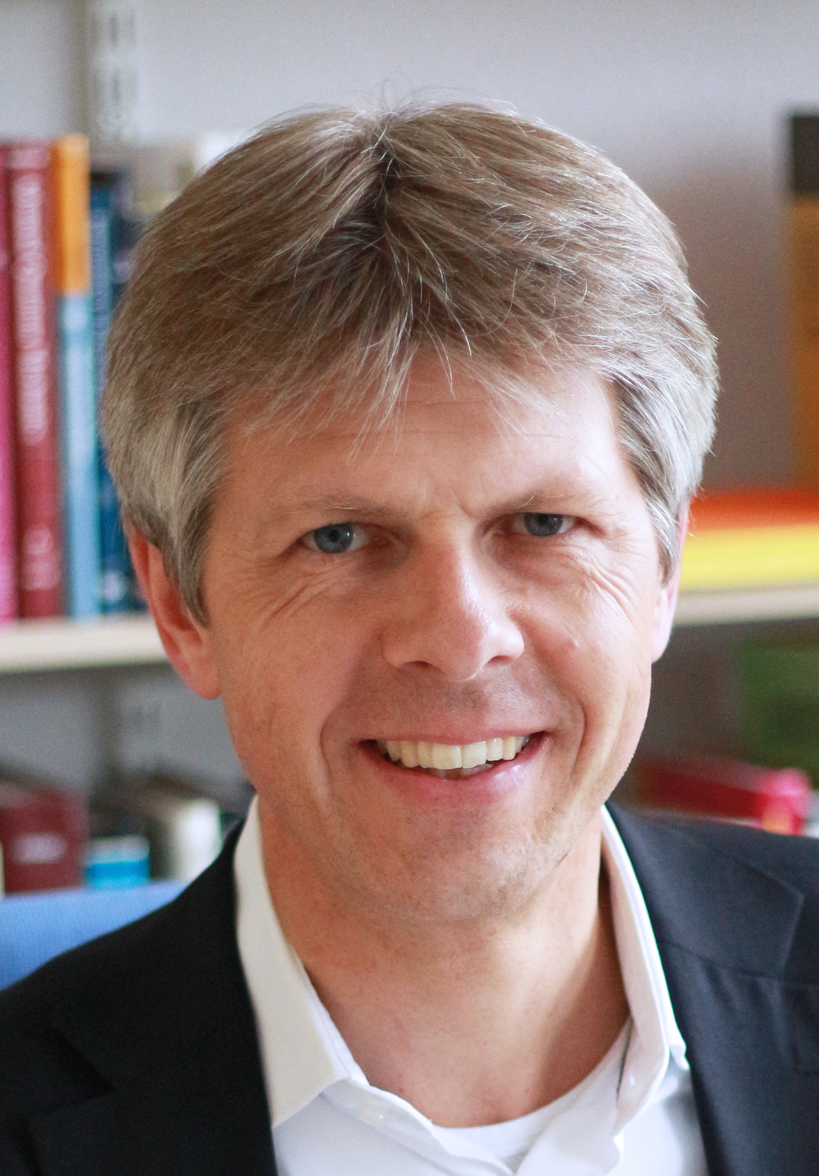
\includegraphics[width=0.8\columnwidth, height=0.25\textheight]{res/vorstellungsfotos/klasen_2016_5.jpg}\\
%\smallskip
%Prof.\ Dr.\ Michael Klasen\\ 
%Institut für Theoretische Physik
%\end{center} 

Herzlich Willkommen an der Universität Münster und insbesondere am Fachbereich Physik! Wir – Ihr 
Lehr-Team für die Physik 1 – möchten Ihnen zu Ihrer Entscheidung, das Physikstudium hier bei uns 
aufzunehmen, gratulieren. Wir freuen uns darauf, mit Ihnen gemeinsam in die spannende, vielfältige 
Welt der Physik einzutauchen und Ihnen dazu die physikalischen und mathematischen Grundlagen zu 
vermitteln. In diesem Semester beschäftigen wir uns hauptsächlich mit den Gebieten Mechanik und 
Spezielle Relativitätstheorie sowie mit mathematischen Methoden, die in der Physik benötigt werden. 
In den nächsten Semestern folgen dann die Module Physik 2 und 3 mit den Themenfeldern 
Thermodynamik, Elektrostatik, Elektrodynamik, Optik und einem ersten kurzen Blick in die 
Quantenmechanik. Unsere Aufgabe ist es hierbei, Ihnen die Physik und die zugehörigen 
Zusammenhänge näherzubringen sowie das „Handwerkszeug“ einzuüben:  die Naturbeobachtung im 
Experiment und die theoretische Beschreibung unter Verwendung der Mathematik als „Sprache der 
Physik“. Die genannten Themenbereiche werden wir mit Ihnen in den Vorlesungen in wechselseitigem 
Bezug von Theorie und Experiment behandeln, Anwendungsbeispiele diskutieren und das Erlernte in 
Übungsgruppen einüben und vertiefen. Den Übungsbetrieb leitet Privatdozent Karol Kovarik. Er 
betreut Sie zusammen mit unseren engagierten Übungsgruppenleiterinnen und -leitern. Für die 
Vorbereitung und Durchführung instruktiver Experimente in der Vorlesung ist Herr Horstmann 
zuständig. 

Damit Sie wissen, mit welchen Dozentinnen und Dozenten Sie es im ersten Semester direkt zu tun 
haben werden, möchten wir uns gerne kurz vorstellen:

Prof.\ Tilmann Kuhn ist für den theoretischen Teil der Vorlesung verantwortlich. Er hat in Stuttgart 
Physik studiert und nach verschiedenen Stationen im In- und Ausland seit 1996 einen Lehrstuhl für 
Theoretische Festkörperphysik in Münster. Mit seiner Arbeitsgruppe untersucht er optische und 
elektronische Eigenschaften sowie dynamische Prozesse in modernen Festkörper-Nanosystemen. 
Häufig in Zusammenarbeit mit experimentellen Gruppen versucht er, durch die Entwicklung von 
theoretischen Modellen ein tieferes physikalisches Verständnis der grundlegenden mikroskopischen 
Prozesse in diesen Materialien zu gewinnen. Einen Schwerpunkt bilden dabei Anwendungen im 
hochaktuellen Gebiet der Quantentechnologien, beispielsweise festkörperbasierte Quellen für 
einzelne Photonen oder Paare von verschränkten Photonen. Hier beschäftigt sich die Arbeitsgruppe 
mit Fragestellungen wie dem Verlust charakteristischer Quanteneigenschaften wie Quantenkohärenz 
und Verschränkung durch Kopplung an die Umgebung und damit, wie dieser Verlust durch geeignete 
Verfahren minimiert werden kann. Neben der Erforschung neuer physikalischer Themen liegt ihm die 
Ausbildung der Studierenden sehr am Herzen. Er war lange Jahre Studiendekan im Fachbereich Physik 
und als solcher für die Organisation der Lehre zuständig. Er freut sich, in diesem Jahr mal wieder, 
zusammen mit den anderen Mitgliedern des Physik-1-Teams, eine neue Kohorte von Studierenden in 
die Arbeitsweise der Physik einzuführen und diese – hoffentlich – für die Physik zu begeistern, so wie 
er selbst immer noch davon begeistert ist. 

Prof.\ Ursula Wurstbauer wird sich um den experimentellen Kursteil kümmern und mit Experimenten, 
zugehörigen Erklärungen und Anwendungsbeispielen den theoretischen Vorlesungsstoff 
veranschaulichen und vertiefen. Zwar ursprünglich Lehramt Mathematik und Physik studiert, ist sie 
von den elektronischen und optischen Eigenschaften von festkörperbasierten Quanten- und 
Nanomaterialien so fasziniert, dass sie bis heute an der Universität geblieben ist. Die Ausbildung von 
jungen Physikerinnen und Physikern sowie angehenden Lehrerinnen und Lehrern in Kombination mit 
faszinierender experimenteller Grundlagenforschung mit Anwendungspotenzial von solarer 
Energiegewinnung über Opto- und Spin Elektronik bis hin zu Quantentechnologie motiviert sie jeden 
Tag. Besonders stolz ist ihre Arbeitsgruppe auf den „kältesten Ort“ in Münster: ein Kühlschrank zur 
Untersuchung von Quantenmaterialien in ihren Laboren. Außerhalb der Uni können Sie Ihre Dozentin 
unterwegs in Münster antreffen: ihre Kinder bei diversen Hobbies begleitend, auf dem Fahrrad, beim 
Joggen oder auch mal bei Schwimmen in der ,,Coburg“. 

Priv.\ Doz.\ Karol Kovarik organisiert den Übungsbetrieb in den Kursen Physik 1-3. Er bietet auch 
verschiedene freiwillige Angebote an, um Ihnen den Einstieg in die Physik zu erleichtern und um Ihnen 
die Gelegenheit zu geben, zusätzliche Fragen zu den Inhalten der Vorlesung und Übungen zu stellen. 
Seit seiner Promotion in 2006 forscht er im Feld der Elementar- und Astroteilchenphysik. Besonders 
spannend findet er die Suche nach der großen vereinheitlichten Theorie und die Frage nach der 
genauen inneren Struktur des Protons. Wenn er nachts nicht schlafen kann, fotografiert er nächtliche 
Landschaften und den Sternenhimmel. 

Das Verständnis komplexer Phänomene und auch die aktuelle Forschung, die uns täglich neu 
überrascht und fasziniert, baut auf den Inhalten der Grundvorlesungen auf, die Sie nun erwarten. Die 
Inhalte werden Sie sich gemeinsam mit Interesse, Motivation und Einsatz erfolgreich selbständig unter 
unserer Anleitung aneignen können. Dazu wünschen wir Ihnen das nötige Durchhaltevermögen, ganz 
viel Freude, stets Erfolg und einen guten Austausch mit Ihren Kommilitonen und Kommilitonen. Physik 
ist kommunikativ und klappt im Team meist besser als beim Einzelkämpfer – auch wenn sie das jetzt (noch) 
nicht nachvollziehen können. Sollten jetzt oder auch im Laufe der Zeit Fragen auftauchen oder Sie 
interessieren sich für unsere Forschungsarbeiten, dann kontaktieren sie uns gerne unter folgenden 
Kontaktdaten: 

\begin{description}
	\item[Prof.\ Dr.\ Tilmann Kuhn:] Institut für Festkörpertheorie, Wilhelm-Klemm-Str.\ 10, Büro 703, Tel. +49 
		251 83-36312, E-Mail: \email{tilmann.kuhn@uni-muenster.de}, \url{https://www.uni-muenster.de/Physik.FT/Forschung/agkuhn/index.html}

	\item[Prof.\ Dr.\ Ursula Wurstbauer:] Physikalisches Institut, Wilhelm-Klemm-Str.\ 10, Büro 506, Tel. +49 251 
		83-33609, E-Mail: \email{wurstbauer@uni-muenster.de}, \url{https://www.uni-muenster.de/Physik.PI/Wurstbauer/index.html}

	\item[Priv.\ Doz.\ Dr.\ Karol Kovarik:] Institut für Theoretische Physik, Wilhelm-Klemm-Str.\ 9, Büro 320, Tel. 
		+49 251 83-34920, E-Mail: \email{karol.kovarik@uni-muenster.de}
\end{description}


\end{multicols}

\vfill

\begin{center}
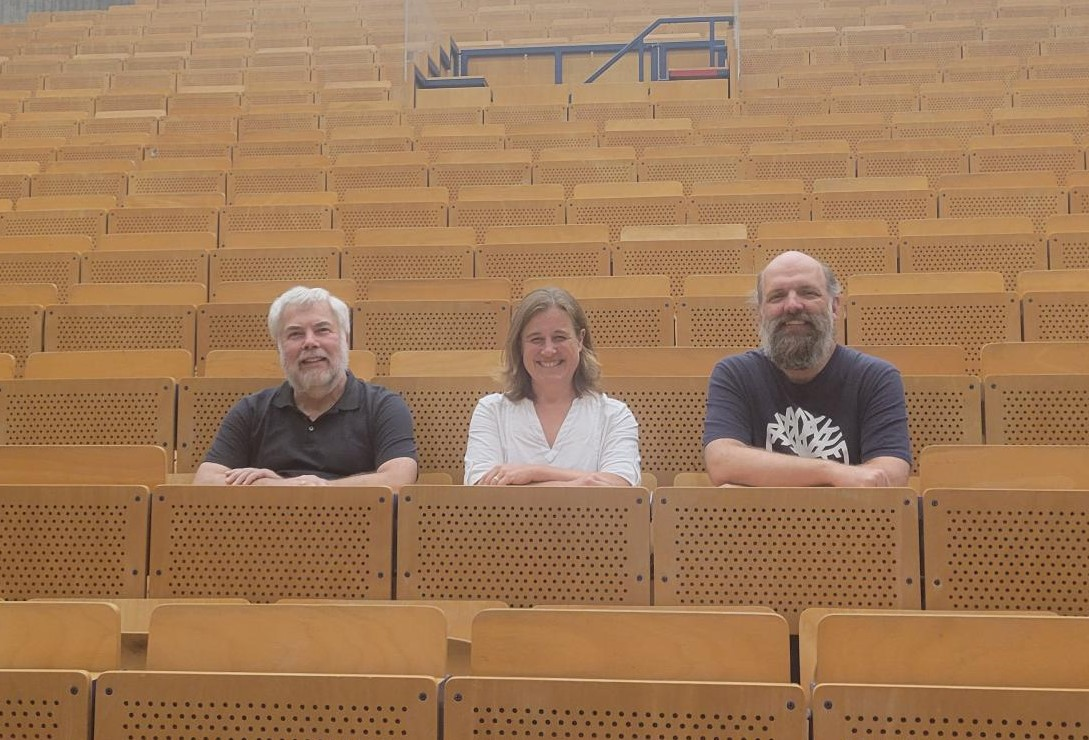
\includegraphics[width=\columnwidth, height=0.35\textheight]{res/ProfsWS2025_cut.jpg}\\
\smallskip
Gruppenfoto des Physik~1-Teams (von links): Tilmann~Kuhn, Ursula~Wurstbauer und Karol~Kovarik.
\end{center}

%\newpage

%\begin{multicols}{2}



%\begin{center}
%\includegraphics[width=0.8\columnwidth]{private/res/comics/manchmal_edited.jpg}\\
%{\footnotesize 
%S.~Harris – \url{sciencecartoonsplus.com}
%}
%\end{center}

%\end{multicols}

%\hspace{\fill}

%\begin{center}
%	\fibelimgtext{
%		\includegraphics[width=0.85\textwidth]{res/xkcd/435_purity.png}
%	}{\url{https://xkcd.com/435}}
% 	%\includegraphics[width=0.85\columnwidth]{private/res/comics/calvin_mathe.pdf}
%\end{center}

%\vfill

\newpage

\begin{multicols}{2}
\begin{center}
	% \includegraphics[width=\columnwidth, height=0.35\textheight]{res/vorstellungsfotos/wend_werner.jpg}\\
	%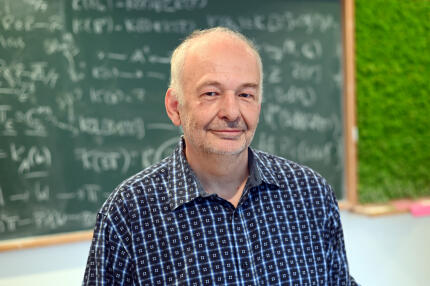
\includegraphics[width=\columnwidth, height=0.35\textheight]{res/vorstellungsfotos/Hille.jpg}\\
	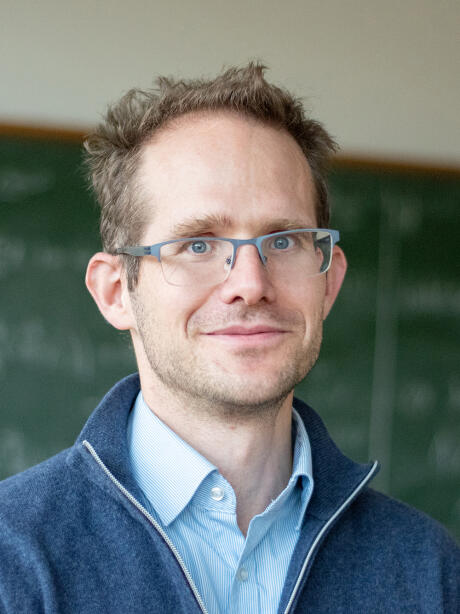
\includegraphics[width=\columnwidth, height=0.35\textheight]{res/GustavHolzegel.jpeg}\\
	\smallskip
 	Prof.\ Dr.\ Gustav Holzegel\\
	Mathematisches Institut
\end{center}
Guten Tag,

mein Name ist Gustav Holzegel und ich werde im WS25/26 die Einführungsvorlesung ,,Mathematik für Studierende der Physik I” lesen. Die Physik ist, spätestens seit Newton, gänzlich in der Sprache der Mathematik formuliert und so ist es wenig verwunderlich, dass eine solide mathematische Ausbildung für Physiker und Physikerinnen unerlässlich ist: Phänomene abstrakt und mathematisch sauber zu formulieren, sowie vielseitige mathematische Werkzeuge parat zu haben, um ,,Dinge auszurechnen” ist geradezu das tägliche Brot! In der Vorlesung werden wir die Grundlagen der Analysis und linearen Algebra behandeln, wie sie auch Studierende der Mathematik in den ersten Semestern erlernen. Das erfordert einen hohen Grad an Abstraktion und viele Stunden eigene Arbeit, um die neuen Konzepte und Methoden zu verinnerlichen. Es ist sicher keine einfache Vorlesung, aber sie öffnet Ihnen hoffentlich die Türen zu vielen spannenden Einsichten in der Physik und der Mathematik.

\[
\resizebox{0.45\hsize}{!}{$\displaystyle\sum_{n = 1}^\infty \frac{1}{n^2} = \frac{\pi^2}{6}$}
\]

Ich persönlich habe übrigens auch vor vielen Jahren mit dem Studium der Physik begonnen, mich dann später immer weiter mathematisch orientiert. Mein eigenes Forschungsgebiet sind heute die partiellen Differentialgleichungen der Allgemeinen Relativitätstheorie, die geradezu ein Musterbeispiel dafür sind, wie Analysis, Geometrie und Physik zusammenhängen und sich gegenseitig befruchten.

Ich freue mich auf ein interessantes Semester mit Ihnen!

\end{multicols}

\vfill

\begin{center}
	\fibelimgtext{
		\includegraphics[width=0.85\textwidth]{res/xkcd/435_purity.png}
	}{\url{https://xkcd.com/435}}
 	%\includegraphics[width=0.85\columnwidth]{private/res/comics/calvin_mathe.pdf}
\end{center}
